% $Id$
%\documentclass[handout]{beamer}
\documentclass{beamer}
\usepackage[utf8]{inputenc}
\usepackage[T1]{fontenc}
\usepackage[english,swedish]{babel}
\usepackage{url}
\usepackage{graphicx}
\usepackage{color}
\usepackage{subfig}
\usepackage{multicol}
\usepackage{amssymb,amsmath,amsthm}
\usepackage{booktabs}
\usepackage[squaren,binary]{SIunits}
\usepackage{algpseudocode}

\setbeamertemplate{bibliography item}[text]
\usepackage[natbib,style=alphabetic,maxbibnames=99]{biblatex}
\addbibresource{bitcoin.bib}

\usepackage{bibsp}

\mode<presentation>{%
  \usetheme{Frankfurt}
  \setbeamercovered{transparent}
  \usecolortheme{seagull}
}
\setbeamertemplate{footline}{\insertframenumber}

\title{%
  Kryptografiska mekanismer och valutor
}
\author{Daniel Bosk\footnote{%
  Detta verk är tillgängliggjort under licensen Creative Commons 
  Erkännande-DelaLika 2.5 Sverige (CC BY-SA 2.5 SE).
	För att se en sammanfattning och kopia av licenstexten besök URL 
	\url{http://creativecommons.org/licenses/by-sa/2.5/se/}.
}}
\institute[MIUN IKS]{%
  %Department of Information and Communication Systems (ICS),\\
  %Mid Sweden University, Sundsvall.
	%
  Avdelningen för informations- och kommunikationssytem (IKS),\\
  Mittuniversitetet, Sundsvall.
}
\date{\today}

%\pgfdeclareimage[height=0.65cm]{university-logo}{MU_logotyp_int_CMYK.pdf}
%\logo{\pgfuseimage{university-logo}}

\AtBeginSection[]{%
  \begin{frame}<beamer>{Översikt}
    \small
    \tableofcontents[currentsection]
  \end{frame}
}

\begin{document}

\begin{frame}
  \titlepage{}
\end{frame}

\begin{frame}{Översikt}
  \tableofcontents{}
\end{frame}


% Since this a solution template for a generic talk, very little can
% be said about how it should be structured. However, the talk length
% of between 15min and 45min and the theme suggest that you stick to
% the following rules:  

% - Exactly two or three sections (other than the summary).
% - At *most* three subsections per section.
% - Talk about 30s to 2min per frame. So there should be between about
%   15 and 30 frames, all told.


% XXX review the approach to bitcoin, perhaps start in the other end?
\section{Kryptografiska valutor -- Bitcoin}

\subsection{Idé}

\begin{frame}{\insertsubsectionhead}
  \begin{itemize}
    \item Decentraliserat, finns ingen central entitet för pålitlighet.
      Använder majoritetsomröstning.
    \item Idén är att alla överföringar är publika i en gemensam 
      överföringshistorik.
    \item Säkerheten baseras på problem som inte enkelt kan lösas.
    \item \emph{Bitcoin miners} löser dessa problem för att skapa bitcoins.
    \item Nya bitcoins skapas kontinuerligt med konstant avtagande hastighet.
    \item Ett bitcoins kan delas i godtyckligt antal delar, och delar kan sedan 
      sättas ihop till större delar.
    \item Överföringar är permanenta.
    \item Låga överföringsavgifter.
  \end{itemize}
\end{frame}

\subsection{Överföringar}

\begin{frame}{\insertsubsectionhead}
  \begin{figure}
    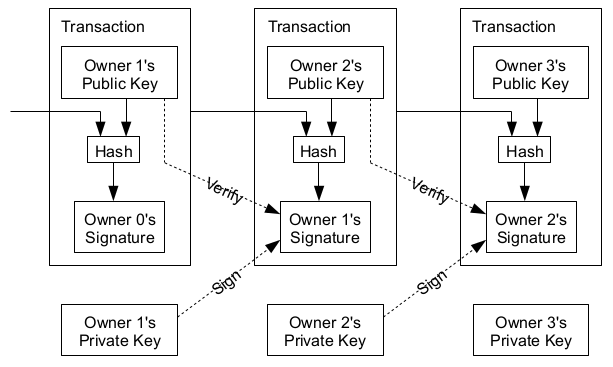
\includegraphics[width=0.7\textwidth]{bitcoin-transfer.png}
    \caption{En överföring från Owner 1 till Owner 2 till Owner 3.
    Bild:~\cite{Nakamoto2008bap}.}
  \end{figure}
\end{frame}

\begin{frame}{\insertsubsectionhead}
  \begin{figure}
    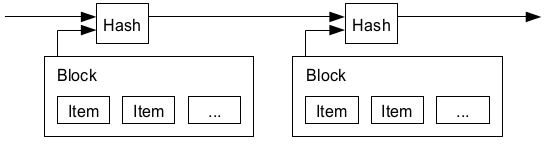
\includegraphics[width=0.7\textwidth]{bitcoin-stamp.png}
    \caption{En enkel tidsstämplingsmekanism.
    Bild:~\cite{Nakamoto2008bap}.}
  \end{figure}
\end{frame}

\begin{frame}{\insertsubsectionhead}
  \begin{itemize}
    \item Behöver kunna förhindra förfalskning.
    \item Den enkla tidsstämplingsmekanismen ger \(h_i = h(h_{i-1}\concat 
      b_i)\), där \(h\) är en kollisionsresistent hashfunktion.
    \item Denna är enkel att förändra.
  \end{itemize}
\end{frame}

\begin{frame}{\insertsubsectionhead}
  \begin{figure}
    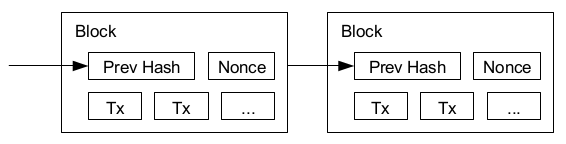
\includegraphics[width=0.7\textwidth]{bitcoin-pow.png}
    \caption{En tidstämplingsmekanism för att förhindra förfalskning.
    Bild:~\cite{Nakamoto2008bap}.}
  \end{figure}
\end{frame}

\begin{frame}{\insertsubsectionhead}
  \begin{itemize}
    \item Det vill säga: \(h_i = h(h_{i-1}\concat b_i\concat n)\), där \(n\) är 
      en nonce.
    \item Svårighetsgraden kontrolleras genom att justera antalet inledande 
      nollor i hashvärdet, det vill säga \(h_i < k\) är ett krav.
    \item Detta är att lösa problemet inversa avbildningen.
    \item Svårighetsgraden \(k\) justeras så att ett sådant problem kan lösas 
      var 10:e minut.
  \end{itemize}
\end{frame}

%\begin{frame}{\insertsubsectionhead}
%  \begin{figure}
%    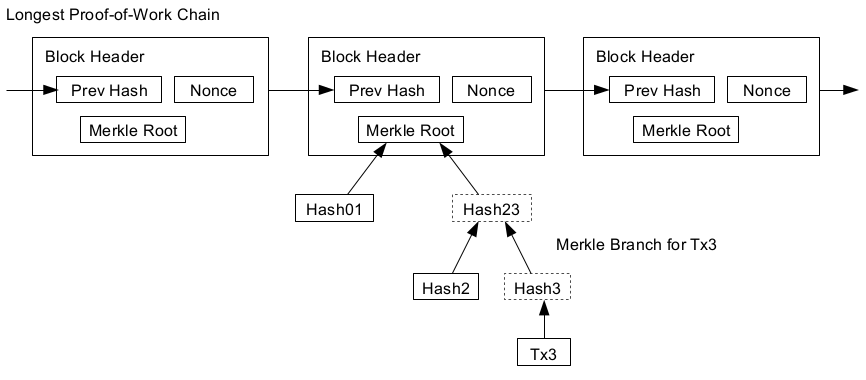
\includegraphics[width=\textwidth]{bitcoin-powchain.png}
%    \caption{En ha med proof-of-work i överföringshistoriken.
%    Bild: \cite{Nakamoto2008bap}.}
%  \end{figure}
%\end{frame}

\subsection{Decentralisering}

\begin{frame}{\insertsubsectionhead}
  \begin{itemize}
    \item Varje överföring sänds till alla deltagande noder.
    \item Varje nod samlar överföringar till ett block.
    \item Varje nod försöker att finna en nonce \(n\) för detta block som 
      uppfyller att \(h_i < k\) för nu gällande \(k\).
    \item När en nod finner detta publiceras det till alla noder i nätverket.
    \item Detta accepteras av noderna om alla transaktioner i blocket inte 
      finns med tidigare i kedjan och hashvärdena stämmer.
    \item Att ett block godtas uttrycks genom att noder utgår från detta block 
      när de skapar nästa block i kedjan.
  \end{itemize}
\end{frame}

\begin{frame}{\insertsubsectionhead}
  \begin{itemize}
    \item Säkerheten kräver att ärliga noder har majoritet.
    \item Alla noder accepterar den längsta existerande kedjan vid eventuella 
      komplikationer.
  \end{itemize}
\end{frame}

% XXX add note on mining networks, e.g. deepbit and BTC guild
% XXX see blockchain.info/pools
%\begin{frame}{\insertsubsectionhead}
%\end{frame}

\subsection{Att dela upp mynt}

\begin{frame}{\insertsubsectionhead}
  \begin{figure}
    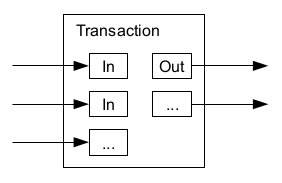
\includegraphics[width=0.4\textwidth]{bitcoin-transaction.png}
    \caption{En bitcoinöverföring.
    Bild:~\cite{Nakamoto2008bap}.}
  \end{figure}
\end{frame}

\subsection{Personlig integritet}

\begin{frame}{\insertsubsectionhead}
  \begin{figure}
    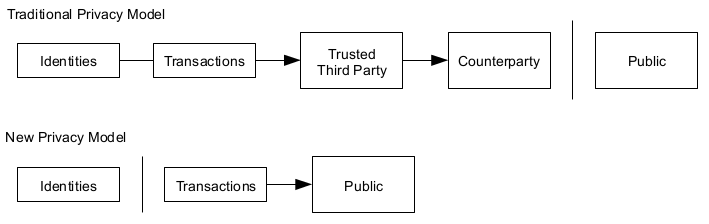
\includegraphics[width=\textwidth]{bitcoin-privacy.png}
    \caption{Bitcoins modell för anonymitet.
    Bild:~\cite{Nakamoto2008bap}.}
  \end{figure}
\end{frame}


%%%%%%%%%%%%%%%%%%%%%%

\begin{frame}[allowframebreaks]{Referenser}
	\small
  \printbibliography{}
\end{frame}

\end{document}
